\TNchapter[Most enterprise benchmarking is theater. A vendor cites a number. Your team underlines it. Nobody asks which version of the test, how many tries, what the test set looked like, or what it cost. This chapter draws the difference between \textit{benchmarking} --- comparing systems on a shared test --- and \textit{evaluation} --- testing your own system on your own job --- and introduces the single most important benchmarking idea in the book: outcome-normalized cost. By the end of this chapter you can read a leaderboard honestly and tell your team what to ask next.]{How you know one agent is better than another}
\label{ch:30-benchmarking-09-strategy}

\begin{figure*}[tb]
\centering
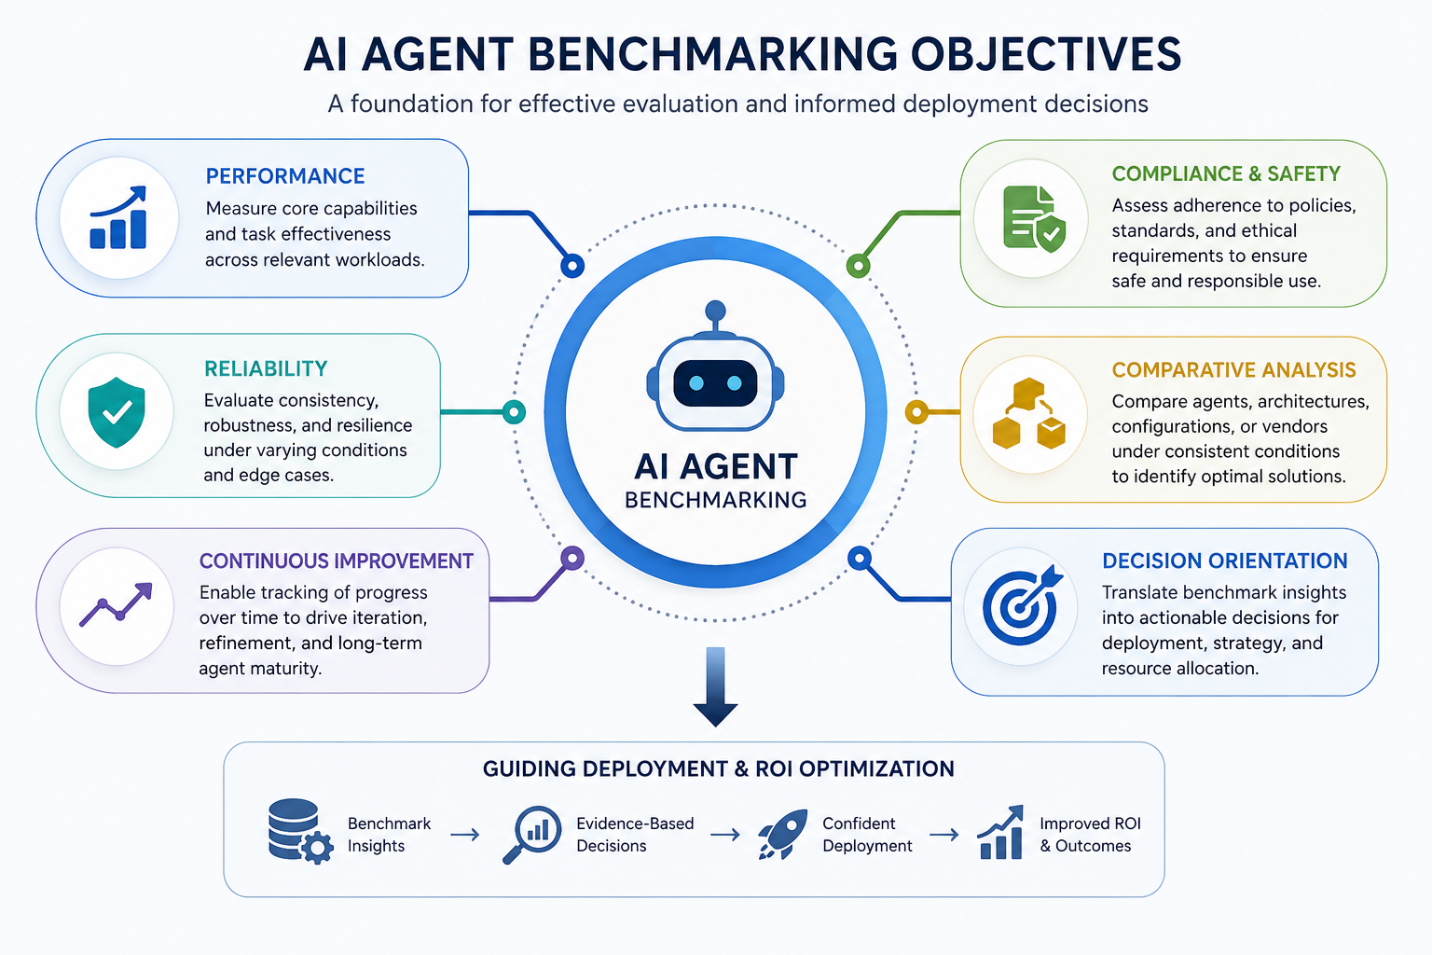
\includegraphics[width=0.9\textwidth]{figures/benchmarking/benchmarking-objectives.png}
\caption{AI agent benchmarking objectives across performance, reliability, compliance, comparative analysis, continuous improvement, and decision orientation.}
\end{figure*}

\starttwocol

\section{The two numbers on the slide}

Two vendors come to Maya's office in the same week. Both want to sell her a customer-service agent. Vendor A's deck claims 92\% task accuracy. Vendor B's deck claims 95\%. Both numbers are bold. Both have footnotes she didn't read. Both teams will quote them to her CFO if she doesn't catch it first.

The two numbers are almost certainly comparing different things. They were measured on different tests, with different rules about how many attempts the agent got, on different data the model may or may not have already seen. Even if both were measured on the same test, the agent that scores 92\% might still be the better one for Aurora --- if its 8\% misses are cheap to recover from and Vendor B's 5\% are not. None of that is on the slide.

This is the chapter that builds the muscle to ask. The rest of Part III gives you the specific techniques. This chapter tells you why none of them matter until your team is asking better questions than the vendors expect.

\section{Benchmark vs. evaluation, in one paragraph}

The two words get used interchangeably in vendor decks. They are not the same thing, and the difference is the spine of Parts III and IV.

\begin{TNdefinition}{Benchmark} a shared, repeatable test that multiple agents run, so you can compare them. A benchmark tells you \textit{how this agent ranks against others}. It says nothing, on its own, about whether the agent will work for your job. \end{TNdefinition}

\begin{TNdefinition}{Evaluation} a test you design for the specific agent doing the specific job you intend it to do. An evaluation tells you \textit{whether this agent does what you hired it to do}. It says nothing about how your agent compares to the field. \end{TNdefinition}

You need both. You need benchmarks to choose between candidates and to spot regressions when the underlying model changes. You need evaluations to know whether the candidate you chose is actually working for your customers. Part III is about the first kind. Part IV is about the second. If you cannot tell which one a vendor is showing you, you cannot make a decision.

\section{Why most benchmarks lie about the agent you'll deploy}

A benchmark score lies in three reliable ways, in roughly this order.

\textbf{First, the benchmark measures a different job than yours.} Public benchmarks are about coding agents in Python, web-browsing agents on synthetic websites, conversational agents in toy domains. Yours is about returns at Aurora, claims triage at Northwind, dispatch at Meridian. A 78\% score on AgentBench tells you the agent can do the things AgentBench tests. It tells you nothing about whether it can navigate your refund policy.

\textbf{Second, the benchmark measures a kinder version of the work than your team will demand.} Most benchmarks run an agent once, on a static test, with full context provided up front. Your team will run the agent multiple times a day, on live data, with context that arrives in pieces. The vendor will quote the easier number. The harder one is the one that matters in production.

\textbf{Third --- and this is the one your team will hate to hear --- the agent may have already seen the test.} Today's frontier LLMs are trained on huge sweeps of the public web. Public benchmarks live on the public web. If the test data leaks into the training data, the benchmark stops measuring capability and starts measuring memorization. The cleanest explanation for why every new model release sets a fresh state-of-the-art on every old benchmark is that the older benchmarks are inside the training data.

\begin{TNdefinition}{Contamination} the situation where the test set has leaked into the model's training data, so the model has effectively seen the answers. There is no clean way to know for sure. The newer the model and the older the benchmark, the more cautious you should be. \end{TNdefinition}

\begin{TNwarning} A score that jumps ten points on a six-month-old benchmark in lockstep with a new model release is more likely contamination than progress. Treat such jumps as a question, not an answer. \end{TNwarning}

\section{Comparative thinking --- the only honest way to read a leaderboard}

The trap in reading a benchmark score is to read it as an absolute. ``85\% accuracy'' sounds like a grade. It is not. Without a baseline, it is a number floating in space.

The number is only useful in comparison. Compared to last year's model, with the same prompt, on the same test? Useful. Compared to a different vendor's product, on the same test, with the same number of attempts? Useful. Compared to nothing? Marketing.

Your team should never report a single benchmark number internally. Every score should sit next to at least two reference points: a baseline (the previous version, or a simple non-agent approach) and a peer (a competing system run under the same conditions). If those reference points don't exist, your team's first job is to produce them. Until then, you are not benchmarking. You are guessing.

\begin{figure*}[tb]
\centering
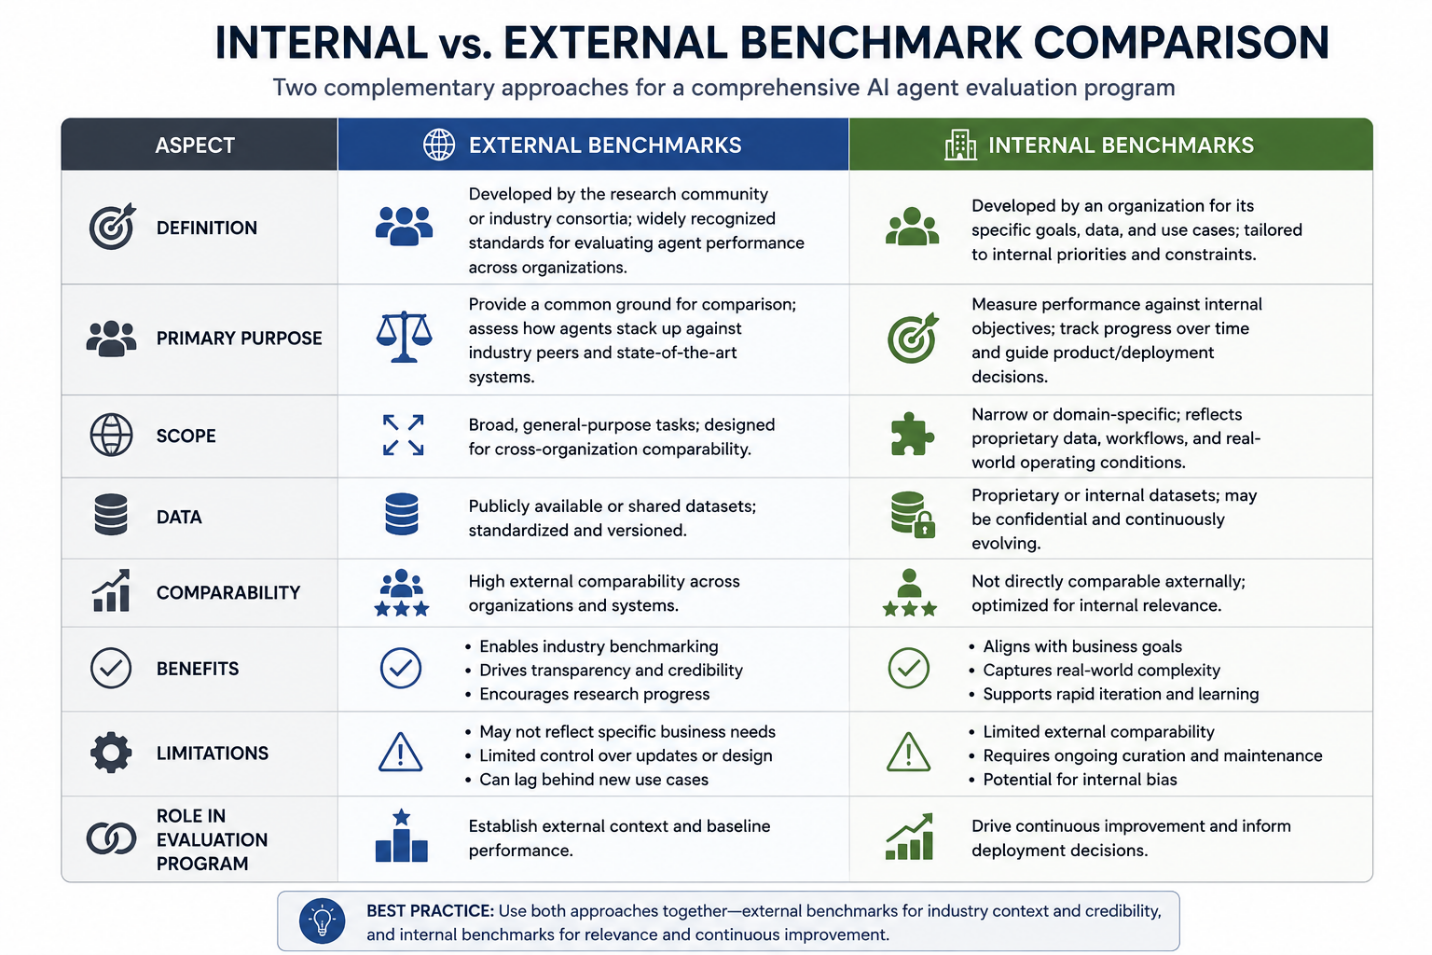
\includegraphics[width=0.9\textwidth]{figures/benchmarking/internal-vs-external.png}
\caption{Internal versus external benchmarks: definition, scope, comparability, and role in evaluation programs.}
\end{figure*}

\section{Outcome-normalized cost --- the framing that survives}

The most important reframe in Part III is this: an agent's quality only matters in proportion to what it costs to produce it. A 95\% agent that costs \$0.70 per resolved ticket is not obviously better than a 92\% agent that costs \$0.30. For a workload of a million tickets a year, the gap between them is \$400,000 --- paid in exchange for three percentage points that may or may not survive contact with your customers.

\begin{TNdefinition}{Outcome-normalized cost} cost per achieved business outcome (a resolved ticket, a closed case, a correct decision), not cost per token or cost per call. The denominator is the work done, not the work attempted. Re-introduced formally in \autoref{ch:30-benchmarking-11-speed-cost}. \end{TNdefinition}

The framing is decision-relevant in three ways. It makes ``good enough at lower cost'' a defensible answer rather than a fudge. It makes accuracy and cost negotiable against each other rather than separate axes that nobody trades. And it forces the question ``how often does this agent succeed cleanly on the first try?'' --- which, more than any single benchmark number, predicts what the agent will feel like to operate.

\begin{TNinpractice}{Cascade Manufacturing} \textit{A manufacturer choosing between two engineering-document Q\&A agents for its plant engineers.} Vendor A quoted 78\% accuracy. Vendor B quoted 82\%. Cascade's procurement lead asked the four questions: which benchmark, what version, how many attempts, on what data. Vendor A's 78\% was on Cascade's own historical document set, single attempt. Vendor B's 82\% was on a public engineering-document benchmark, with three attempts allowed. Cost-per-resolved-query, including the human review time each system's misses required, made Vendor A cheaper by 40\%. Cascade bought from A and used the gap to fund three months of internal evaluation work. \end{TNinpractice}

\section{Statistical sanity for benchmarking}

Two benchmark numbers are different. Are they meaningfully different? Most teams don't ask, and most decisions get made on noise.

A benchmark score is an estimate. Run the same agent against the same benchmark twice and you'll likely get different numbers. The variance comes from sampling-based decoding, from how the prompts were ordered, from which hardware ran the job, and from a dozen smaller sources. A three-percentage-point difference between two agents may be a real difference or may be the noise floor. Your team needs the discipline to tell which.

The discipline has three parts. First, run multiple trials with different random seeds --- three to five at minimum, more if the decision is consequential. Second, report a confidence interval, not just a point estimate; ``82\%, with a 95\% interval of 79--85\%'' is honest, while ``82\%'' alone is not. Third, when comparing two agents, ask whether their intervals overlap. If they do, the difference may not be real, and ``the better one'' is a coin flip.

\begin{TNdefinition}{Bootstrap confidence interval} a way of estimating the uncertainty in a benchmark score by resampling the test cases many times (with replacement) and recomputing the score each time. The middle 95\% of those scores is your confidence interval. What this means for your decision: if two agents' intervals overlap, you do not yet have evidence that one is better; you need more data, not a stronger opinion. \end{TNdefinition}

Significance tests --- t-tests, Mann-Whitney U, permutation tests --- turn the ``do their intervals overlap'' intuition into a number. Effect sizes (Cohen's d) tell you whether the difference, if real, is large enough to matter. The math lives in \autoref{ch:30-benchmarking-12-comparing}; the discipline lives here. If your team reports two scores side by side without an interval, ask them to redo the work.

\section{What Part III gives you}

The rest of this Part teaches your team to read benchmarks honestly. \autoref{ch:30-benchmarking-10-capability} walks the five public benchmarks they will see in vendor decks --- AgentBench, SWE-bench Verified, $\tau$-bench, GAIA, HELM --- and tells them what each one actually measures. \autoref{ch:30-benchmarking-11-speed-cost} handles the operational benchmarks your CFO will care about: latency, throughput, and outcome-normalized cost as a worked example. \autoref{ch:30-benchmarking-12-comparing} covers what changes when ``benchmark once'' becomes ``benchmark every release'' --- regression detection, leaderboard gaming, and the statistical methods that keep your team honest over time.

Part III stops at the boundary of ``compared to peers.'' When you need ``fit for our job,'' you are in the territory of evaluation. That is Part IV.

\TNrule

\stoptwocol

\begin{TNkeytakeaways}
\item Benchmarks compare; evaluations answer. Vendors mostly show benchmarks. Your job is to know which you're being shown.
\item A single benchmark number means nothing without a baseline and a peer reference. Numbers in isolation are marketing.
\item The score that wins is rarely the highest one. It is the one with the lowest cost per resolved outcome.
\item Contamination is real, unmeasurable, and the most likely explanation for suspiciously fresh state-of-the-art results.
\item A three-point difference is noise until proven otherwise. Confidence intervals are the proof.
\end{TNkeytakeaways}

\begin{TNchecklist}
\item For every benchmark number on a vendor's deck, demand which benchmark, which version, how many attempts, on what data.
\item Require every internal benchmark report to include a baseline and at least one peer comparison.
\item Make outcome-normalized cost --- dollars per resolved ticket, not per token --- the headline metric in every agent decision.
\item Reject single-point estimates. Require confidence intervals or score distributions across multiple trials.
\item Build the team habit of asking ``could the test be in the training data?'' before celebrating a fresh state-of-the-art.
\item Reserve a benchmark slot in every quarterly review for the question ``what changed since last quarter, and is the change real?''
\end{TNchecklist}



